%%%%%%%%%%%%%%%%%%%%%%%%%%%%%%%%%%%%%%%%%%%%%%%%%%%%%%%
\documentclass{article}
%%%%%%%%%%%%%%%%%%%%%%%%%%%%%%%%%%%%%%%%%%%%%%%%%%%%%%%
\usepackage[utf8]{vietnam}
%%%%%%%%%%%%%%%%%%%%%%%%%%%%%%%%%%%%%%%%%%%%%%%%%%%%%%%
\usepackage{graphicx}
%%%%%%%%%%%%%%%%%%%%%%%%%%%%%%%%%%%%%%%%%%%%%%%%%%%%%%%
\usepackage{hyperref}
%%%%%%%%%%%%%%%%%%%%%%%%%%%%%%%%%%%%%%%%%%%%%%%%%%%%%%%
\usepackage{xcolor}
\pagecolor[RGB]{40, 42, 54} % Đặt màu nền
\color[RGB]{18, 161, 24} % Đặt màu chữ
%%%%%%%%%%%%%%%%%%%%%%%%%%%%%%%%%%%%%%%%%%%%%%%%%%%%%%%
\usepackage{float} % Cố định hình ảnh [H]
%%%%%%%%%%%%%%%%%%%%%%%%%%%%%%%%%%%%%%%%%%%%%%%%%%%%%%%
\begin{document}
%%%%%%%%%%%%%%%%%%%%%%%%%%%%%%%%%%%%%%%%%%%%%%%%%%%%%%%
\tableofcontents
\newpage
%%%%%%%%%%%%%%%%%%%%%%%%%%%%%%%%%%%%%%%%%%%%%%%%%%%%%%%
\listoffigures
\newpage
%%%%%%%%%%%%%%%%%%%%%%%%%%%%%%%%%%%%%%%%%%%%%%%%%%%%%%%
\section{Tuần 4: Power Query và Xây dựng Mô hình}
%%%%%%%%%%%%%%%%%%%%%%%%%%%%%%%%%%%%%%%%%%%%%%%%%%%%%%%
\subsection{Bài 1}
%%%%%%%%%%%%%%%%%%%%%%%%%%%%%%%%%%%%%%%%%%%%%%%%%%%%%%%
\subsubsection{Video 1}

% \caption{Hướng dẫn extract dữ liệu từ file Excel}
% ![alt text](Bai1/Video1/HuongDan/0.png)
% \caption{Hướng dẫn extract dữ liệu từ folder}
% ![alt text](Bai1/Video1/HuongDan/1.png)
% \caption{Hướng dẫn extract dữ liệu từ Google sheet}
% ![alt text](Bai1/Video1/HuongDan/2.png)
% \caption{Hướng dẫn extract dữ liệu từ CSDL}
% ![alt text](Bai1/Video1/HuongDan/3.png)

% \caption{Thực hành extract dữ liệu từ CSV}
% ![alt text](Bai1/Video1/ThucHanh/0.png)
% \caption{Thực hành extract dữ liệu từ TXT}
% ![alt text](Bai1/Video1/ThucHanh/1.png)
% \caption{Thực hành extract dữ liệu từ MySQL}
% ![alt text](Bai1/Video1/ThucHanh/2.png)
%%%%%%%%%%%%%%%%%%%%%%%%%%%%%%%%%%%%%%%%%%%%%%%%%%%%%%%
\subsubsection{Video 2}

% \caption{Hướng dẫn chuyển đổi dữ liệu Merge Query}
% ![alt text](Bai1/Video2/HuongDan/0.png)
% \caption{Hướng dẫn chuyển đổi dữ liệu Append Query}
% ![alt text](Bai1/Video2/HuongDan/1.png)
% \caption{Hướng dẫn chuyển đổi dữ liệu Group by}
% ![alt text](Bai1/Video2/HuongDan/2.png)
% \caption{Hướng dẫn chuyển đổi dữ liệu Unpivot}
% ![alt text](Bai1/Video2/HuongDan/3.png)
% \caption{Hướng dẫn chuyển đổi dữ liệu Tranpose}
% ![alt text](Bai1/Video2/HuongDan/4.png)
% \caption{Hướng dẫn chuyển đổi dữ liệu Pivot}
% ![alt text](Bai1/Video2/HuongDan/5.png)

% \caption{Thực hành kết hợp: Tranpose, Pivot, Unpivot}
% ![alt text](Bai1/Video2/ThucHanh/0.png)
%%%%%%%%%%%%%%%%%%%%%%%%%%%%%%%%%%%%%%%%%%%%%%%%%%%%%%%
\subsubsection{Video 3}




\begin{figure}[H]
    \centering
    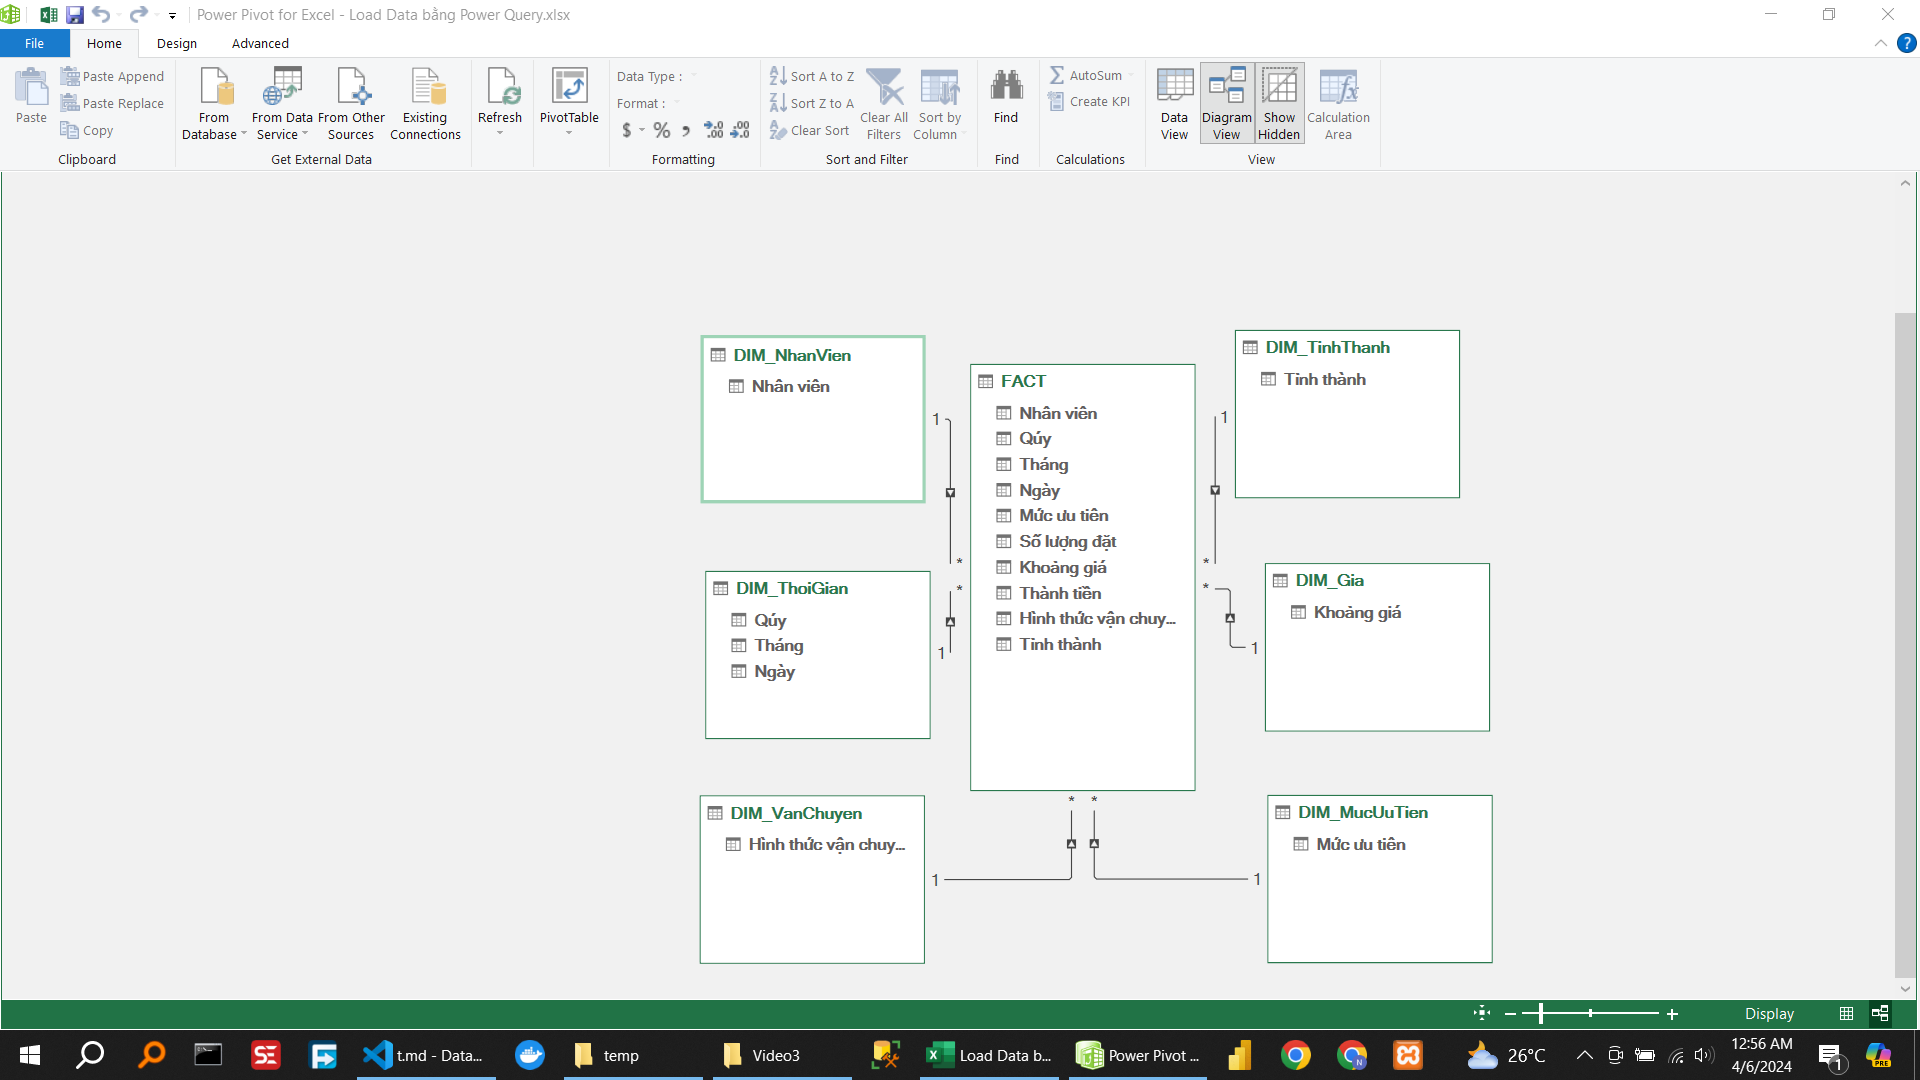
\includegraphics[scale = 0.15]{Bai1/Video3/HuongDan/0.png}
    \caption{Hướng dẫn Load dữ liệu và xây dựng Data Model}
\end{figure}



\textbf{Câu hỏi:} Dim và Fact: Bảng nào là dữ liệu động, bảng nào là dữ liệu tĩnh?

\begin{itemize}
    \item  Dim là bảng dữ liệu tĩnh. Dim cung cấp các thông tin, ngữ cảnh cho bảng Fact.
    \item   Fact là bảng dữ liệu động. Fact Có độ đo có thể tính toán được dựa trên các Dim.
\end{itemize}

\textbf{Câu hỏi:}   Có những dạng data model nào?

Những dạng data model phổ biến bao gồm:

\begin{itemize}
    \item  Mô hình dữ liệu quan hệ: Dữ liệu được tổ chức thành các bảng có mối quan hệ với nhau thông qua các khóa chính và khóa ngoại.
    \item   Mô hình dữ liệu đa chiều: Dữ liệu được tổ chức thành các bảng chi tiết và bảng số liệu, tạo nên một không gian dữ liệu đa chiều để phân tích.
    \item    Mô hình dữ liệu đồ thị: Dữ liệu được biểu diễn dưới dạng đồ thị với các đỉnh và cạnh để mô tả mối quan hệ giữa các đối tượng.
\end{itemize}

%%%%%%%%%%%%%%%%%%%%%%%%%%%%%%%%%%%%%%%%%%%%%%%%%%%%%%%
\subsubsection{Video 4}

%%%%%%%%%%%%%%%%%%%%%%%%%%%%%%%%%%%%%%%%%%%%%%%%%%%%%%%
\subsubsection{Video 5}

%%%%%%%%%%%%%%%%%%%%%%%%%%%%%%%%%%%%%%%%%%%%%%%%%%%%%%%
\subsection{Bài 2}

% \caption{Thực hành xây dựng luồng nghiệp vụ (Business flow)}
% ![alt text](Bai2/ThucHanh/Business-flow.png)
% \caption{Thực hành xây dựng dòng dữ liệu giữa các hệ thống (Data flow)}
% ![alt text](Bai2/ThucHanh/Data-flow.png)
% \caption{Thực hành xây dựng kiến trúc hệ thống phân tích dữ liệu}
% ![alt text](Bai2/ThucHanh/Architecture.png)

%%%%%%%%%%%%%%%%%%%%%%%%%%%%%%%%%%%%%%%%%%%%%%%%%%%%%%%
\end{document}
%%%%%%%%%%%%%%%%%%%%%%%%%%%%%%%%%%%%%%%%%%%%%%%%%%%%%%%


